% ---------------------------------------------------------------
% DAS Cit-Ihlali Siniflandirmasi -- Gercek Saha Verisi Sonuclari
%
% Derleme:
%     pdflatex rapor.tex
%
% Not: babel/turkish BILEREK kullanilmiyor. babel'in Turkce modulu
% ':' ve '=' gibi karakterleri etkin (active) hale getirir ve bu,
% matematik modunda ya da URL'lerde beklenmedik hatalara yol acar.
% T1 + utf8 Turkce karakterleri zaten dogru basiyor.
% ---------------------------------------------------------------
\documentclass[11pt,a4paper]{article}

\usepackage[utf8]{inputenc}
\usepackage[T1]{fontenc}
\usepackage{lmodern}
\usepackage[a4paper,margin=2.2cm]{geometry}
\usepackage{graphicx}
\usepackage{float}
\usepackage{caption}
\usepackage{subcaption}
\usepackage{booktabs}
\usepackage{microtype}

\captionsetup{font=small,labelfont=bf,skip=4pt}
\setlength{\parskip}{0.5em}
\setlength{\parindent}{0pt}
% Sekiller arasi/uzeri bosluklari kis -- her sey 2 sayfaya sigsin
\setlength{\textfloatsep}{8pt plus 2pt minus 2pt}
\setlength{\intextsep}{8pt plus 2pt minus 2pt}
\setlength{\floatsep}{8pt plus 2pt minus 2pt}

\begin{document}

\begin{center}
  {\LARGE\bfseries DAS Tabanlı Çit-İhlali Sınıflandırması}\\[3pt]
  {\large Gerçek Saha Verisi ile Eğitim Sonuçları}
\end{center}
\vspace{0.4em}

Gerçek saha verisiyle eğitilen 2D-CNN + SK-Attention modeli, ayrı tutulan
test setinde macro-F1 0.874 (doğruluk 0.839) elde etti ve aşılması hedeflenen
taban çizgisini (elle çıkarılmış 26 özellik üzerinde doğrusal sınıflandırıcı,
macro-F1 0.771) 0.103 puan geçti. Model 220.834 eğitim penceresiyle eğitildi;
bu pencereler 21.101 bağımsız kayıt dosyasından geliyor ve bölmeler dosya,
oturum ve tarih düzeyinde çakışmasız olduğu doğrulanmış durumda. Sınıf bazında
sonuçlar: \texttt{noise} F1 0.977, \texttt{climbing} 0.851, \texttt{cutting}
0.794. Kazancın tamamı \texttt{climbing} ve \texttt{cutting} sınıflarında
toplanıyor (taban çizgisine göre sırasıyla +0.198 ve +0.116); \texttt{noise}
sınıfı taban çizgisinde de çözülmüş durumdaydı ve orada değişim yok. Bu,
Faz 0 denetiminin öngörüsünü doğruluyor: tek tek ölçülen elle çıkarılmış
özellikler \texttt{climbing} ile \texttt{cutting}'i ayıramıyordu, ancak
spektrogramın tamamını gören evrişimli bir model bu ayrımı büyük ölçüde
yapabiliyor. Kalan hata da hâlâ aynı çiftte yoğunlaşıyor --- \texttt{cutting}
örneklerinin \%24'ü \texttt{climbing}, \texttt{climbing} örneklerinin \%11.7'si
\texttt{cutting} olarak sınıflandırılıyor; \texttt{noise} ise 3.554 örnekten
yalnızca 84'ünde karışıyor. Eğitim 29 epoch sürdü (en iyi epoch 23, doğrulama
macro-F1 izlenerek seçildi) ve 102 dakika aldı; test setine yalnızca bir kez,
model seçimi tamamlandıktan sonra bakıldı.

\begin{figure}[H]
  \centering
  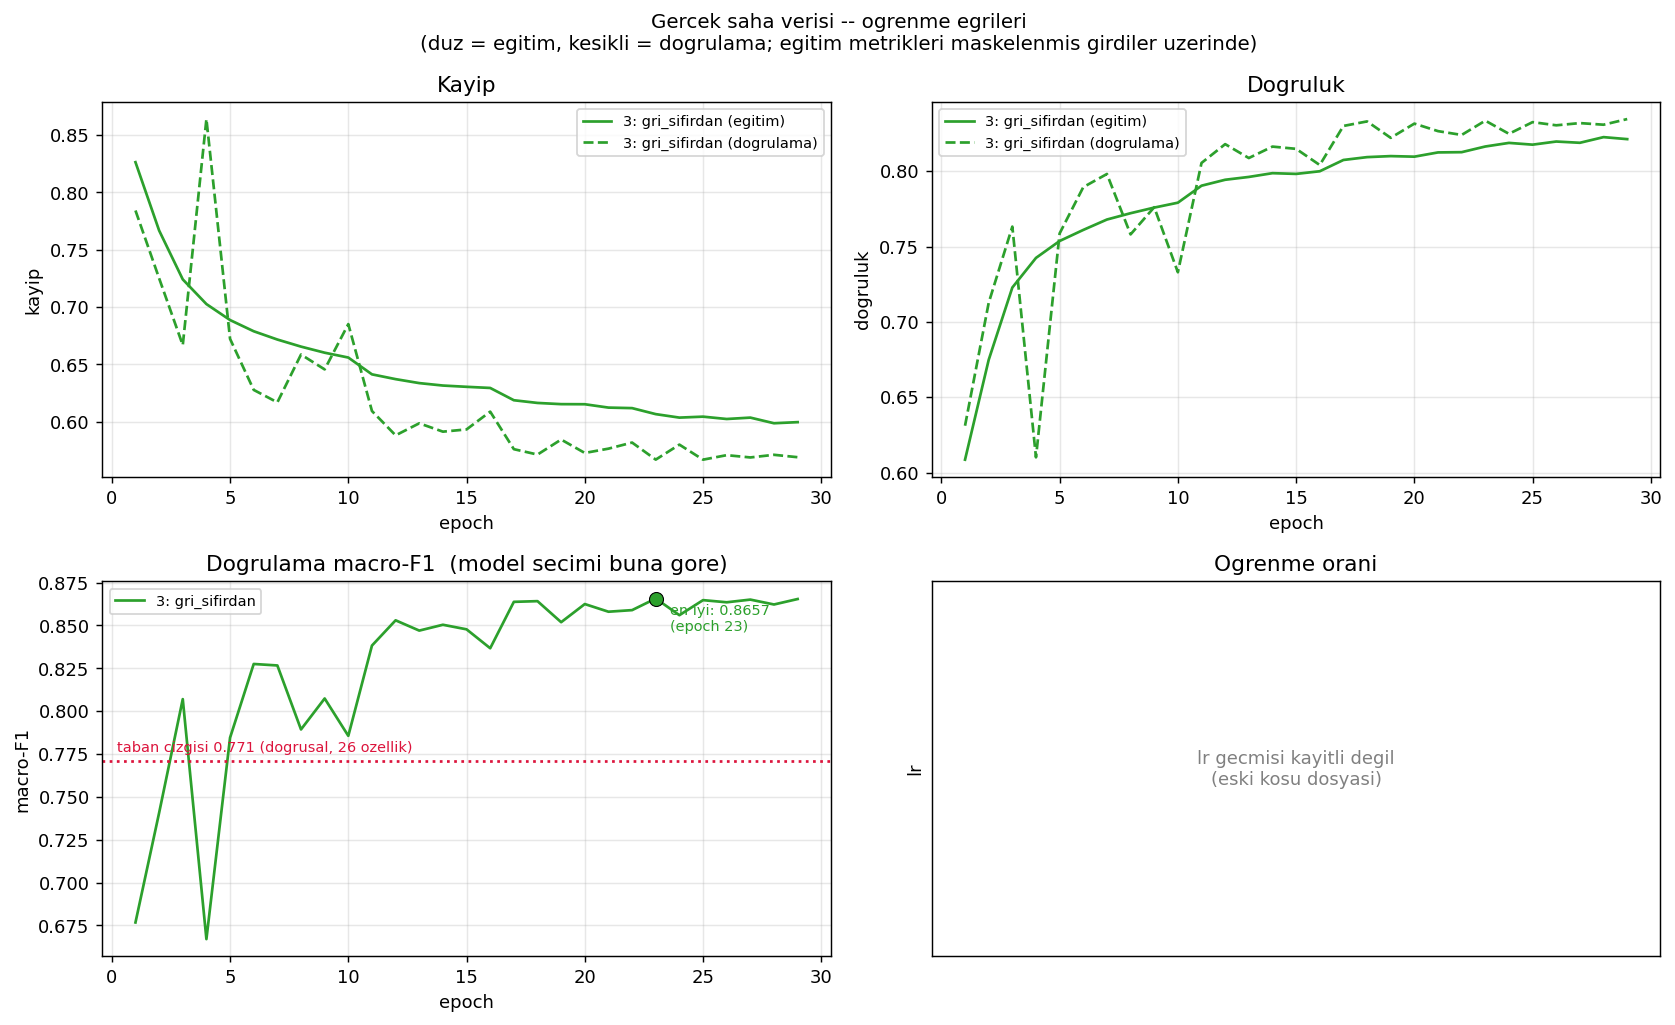
\includegraphics[width=0.97\textwidth]{ogrenme_egrileri.png}
  \caption{Öğrenme eğrileri. Düz çizgi eğitim, kesikli çizgi doğrulama.
  Eğitim metrikleri maskelenmiş girdiler üzerinde ölçüldüğü için doğrulama
  eğrisinin üstte seyretmesi beklenen bir durumdur ve aşırı öğrenme
  olmadığına işaret eder (en iyi epoch'ta eğitim--doğrulama doğruluk farkı
  $-0.017$). Kırmızı kesikli çizgi taban çizgisidir (0.771).}
  \label{fig:egriler}
\end{figure}

\begin{figure}[H]
  \centering
  \begin{subfigure}[b]{0.52\textwidth}
    \centering
    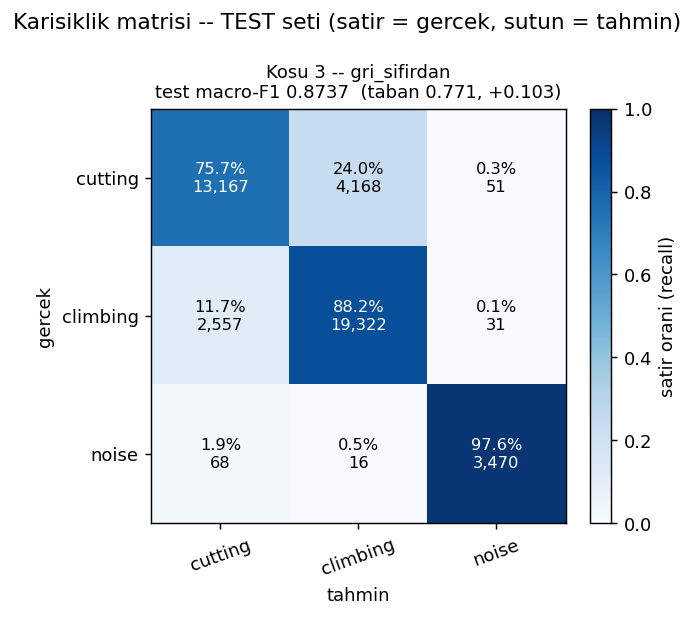
\includegraphics[width=\textwidth]{karisiklik_matrisi.png}
    \caption{Test seti karışıklık matrisi (satır: gerçek, sütun: tahmin).
    Renk ölçeği satır bazında normalize edilmiştir, yani hücre rengi o
    sınıfın recall değerini yansıtır; ham sayıyla renklendirmek örnek
    sayısı az olan \texttt{noise} sınıfını yanıltıcı biçimde soluk
    gösterirdi. Hücrelerde hem satır yüzdesi hem ham sayı verilmiştir.}
    \label{fig:karisiklik}
  \end{subfigure}\hfill
  \begin{subfigure}[b]{0.44\textwidth}
    \centering
    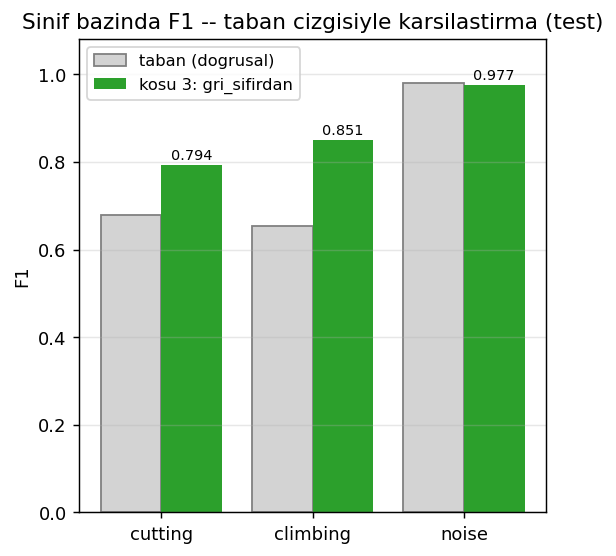
\includegraphics[width=\textwidth]{sinif_bazinda_f1.png}
    \caption{Sınıf bazında F1 değerlerinin taban çizgisiyle
    karşılaştırması. Kazancın \texttt{climbing} ve \texttt{cutting}
    sınıflarında toplandığı, \texttt{noise} sınıfında ise taban çizgisinin
    zaten tavana yakın olduğu görülüyor.}
    \label{fig:sinif}
  \end{subfigure}
\end{figure}

\end{document}
